% !TEX encoding = UTF-8 Unicode
\documentclass[a4paper,12pt]{article}
	
	% В этом документе преамбула
	
	%%% Работа с русским языком
	\usepackage{cmap}					% поиск в PDF
	\usepackage{mathtext} 				% русские буквы в формулах
	\usepackage[T2A]{fontenc}			% кодировка
	\usepackage[utf8]{inputenc}			% кодировка исходного текста
	\usepackage[english]{babel}	% локализация и переносы
	\usepackage{indentfirst}
	\frenchspacing
	
	\renewcommand{\epsilon}{\ensuremath{\varepsilon}}
	\renewcommand{\phi}{\ensuremath{\varphi}}
	\renewcommand{\kappa}{\ensuremath{\varkappa}}
	\renewcommand{\le}{\ensuremath{\leqslant}}
	\renewcommand{\leq}{\ensuremath{\leqslant}}
	\renewcommand{\ge}{\ensuremath{\geqslant}}
	\renewcommand{\geq}{\ensuremath{\geqslant}}
	\renewcommand{\emptyset}{\varnothing}
	
	%%% Дополнительная работа с математикой
	\usepackage{amsmath,amsfonts,amssymb,amsthm,mathtools} % AMS
	\usepackage{icomma} % "Умная" запятая: $0,2$ --- число, $0, 2$ --- перечисление
	
	%% Номера формул
	%\mathtoolsset{showonlyrefs=true} % Показывать номера только у тех формул, на которые есть \eqref{} в тексте.
	%\usepackage{leqno} % Нумереация формул слева
	
	%% Свои команды
	\DeclareMathOperator{\sgn}{\mathop{sgn}}
	
	%% Перенос знаков в формулах (по Львовскому)
	\newcommand*{\hm}[1]{#1\nobreak\discretionary{}
		{\hbox{$\mathsurround=0pt #1$}}{}}
	
	%%% Работа с картинками
	\usepackage{graphicx}  % Для вставки рисунков
	\setlength\fboxsep{3pt} % Отступ рамки \fbox{} от рисунка
	\setlength\fboxrule{1pt} % Толщина линий рамки \fbox{}
	\usepackage{wrapfig} % Обтекание рисунков текстом
	
	%%% Работа с таблицами
	\usepackage{array,tabularx,tabulary,booktabs} % Дополнительная работа с таблицами
	\usepackage{longtable}  % Длинные таблицы
	\usepackage{multirow} % Слияние строк в таблице
	
	%%% Теоремы
	\theoremstyle{plain} % Это стиль по умолчанию, его можно не переопределять.
	\newtheorem{theorem}{Theorem}
	\newenvironment{Proof} % имя окружения
	{\par\noindent{\bf Proof.}} % команды для \begin
	{\hfill$\scriptstyle\blacksquare$} % команды для \end
	
	\newtheorem{proposition}[theorem]{Утверждение}
	
	\theoremstyle{definition} % "Определение"
	\newtheorem{corollary}{Следствие}[theorem]
	\newtheorem{problem}{Задача}[section]
	
	\theoremstyle{remark} % "Примечание"
	\newtheorem*{nonum}{Решение}
	
	%%% Программирование
	\usepackage{etoolbox} % логические операторы
	
	%%% Страница
	\usepackage{extsizes} % Возможность сделать 14-й шрифт
	\usepackage{geometry} % Простой способ задавать поля
	\geometry{top=25mm}
	\geometry{bottom=35mm}
	\geometry{left=35mm}
	\geometry{right=20mm}
	%
	%\usepackage{fancyhdr} % Колонтитулы
	% 	\pagestyle{fancy}
	%\renewcommand{\headrulewidth}{0pt}  % Толщина линейки, отчеркивающей верхний колонтитул
	% 	\lfoot{Нижний левый}
	% 	\rfoot{Нижний правый}
	% 	\rhead{Верхний правый}
	% 	\chead{Верхний в центре}
	% 	\lhead{Верхний левый}
	%	\cfoot{Нижний в центре} % По умолчанию здесь номер страницы
	
	\usepackage{setspace} % �?нтерлиньяж
	%\onehalfspacing % �?нтерлиньяж 1.5
	%\doublespacing % �?нтерлиньяж 2
	%\singlespacing % �?нтерлиньяж 1
	
	\usepackage{lastpage} % Узнать, сколько всего страниц в документе.
	
	\usepackage{soul} % Модификаторы начертания
	
	\usepackage{hyperref}
	\usepackage[usenames,dvipsnames,svgnames,table,rgb]{xcolor}
	\hypersetup{				% Гиперссылки
		unicode=true,           % русские буквы в раздела PDF
		pdftitle={Заголовок},   % Заголовок
		pdfauthor={Автор},      % Автор
		pdfsubject={Тема},      % Тема
		pdfcreator={Создатель}, % Создатель
		pdfproducer={Производитель}, % Производитель
		pdfkeywords={keyword1} {key2} {key3}, % Ключевые слова
		colorlinks=true,       	% false: ссылки в рамках; true: цветные ссылки
		linkcolor=red,          % внутренние ссылки
		citecolor=black,        % на библиографию
		filecolor=magenta,      % на файлы
		urlcolor=blue           % на URL
	}
	
	\usepackage{csquotes} % Еще инструменты для ссылок
	
	%\usepackage[style=authoryear,maxcitenames=2,backend=biber,sorting=nty]{biblatex}
	
	\usepackage{multicol} % Несколько колонок
	
	\usepackage{tikz} % Работа с графикой
	\usepackage{pgfplots}
	\usepackage{pgfplotstable}
	\usepackage{caption}
	\usepackage{subcaption}
	
	\usepackage{algorithm}
	\usepackage[noend]{algcompatible}
	
	\newcommand{\ba}{\mathbf{a}}
	\newcommand{\bb}{\mathbf{b}}
	\newcommand{\bw}{\mathbf{w}}
	\newcommand{\by}{\mathbf{y}}
	\newcommand{\bx}{\mathbf{x}}
	\newcommand{\bz}{\mathbf{z}}
	\newcommand{\cA}{\mathcal{A}}
	\newcommand{\bJ}{\mathbf{J}}
	\newcommand{\bQ}{\mathbf{Q}}
	\newcommand{\bbC}{\mathbb{C}}
	\newcommand{\bbR}{\mathbb{R}}
	\newcommand{\bbY}{\mathbb{Y}}
	\newcommand{\bW}{\mathbf{W}}
	\newcommand{\bH}{\mathbf{H}}
	\newcommand{\bF}{\mathbf{F}}
	\newcommand{\bR}{\mathbf{R}}
	\newcommand{\bX}{\mathbf{X}}
	
	\newcommand{\T}{{\text{\tiny\sffamily\upshape\mdseries T}}}
	\newcommand{\argmin}{\mathop{\arg \min}\limits}
	\newcommand{\argmax}{\mathop{\arg \max}\limits}
	
	\usepackage{tikz-cd}
	
	\begin{document}
		
	\section*{Problem Statement}

	We consider the problem of predicting an target variable $y \in \bbY$ given an object $\bx \in \bbR^{n}$. The space~$\bbY = \{0, 1\}$ for binary classification problem and $\bbY = \bbR$ for regression problem.
	The goal is to build a model $f(\bx | \bw), \bw \in \mathbb{R}^p$ which outcomes a prediction for each object.
	There are given the design matrix~$\bX = [\bx_1, \dots, \bx_m]^{\T} \in \bbR^{m \times n}$ and the target vector~$\by = [y_1, \dots, y_m]^{\T} \in \bbY^{m}$. 
	The goal is to find the optimal weight vector $\bw^*$.
	The weights~$\bw$ are fitted by the minimization of an error function:
	\begin{equation}
	\bw^* = \argmin_{\bw \in \bbR^p} S(\bw | \bX, \by, f).
	\label{eq:error_function}
	\end{equation}
	The investigated choices for the error function~$S(\bw | \bX, \by, f)$ are
	squared error for regression problem: 
		\begin{equation}
			S(\bw | \bX, \by, f) = \frac 12 \| \by - \mathbf{f}(\bX | \bw) \|_2^2 = \frac 12 \sum_{i=1}^m \| y_i - f(\bx_i | \bw)\|^2;
			\label{eq:squared_error}
		\end{equation}
	cross-entropy for classification problem: 
		\begin{equation}
			S(\bw | \bX, \by, f) = \sum_{i=1}^m \bigl[y_i \log f (\bx_i | \bw) + (1-y_i) \log (1 - f (\bx_i | \bw))\bigr].
			\label{eq:log_loss}
		\end{equation}
	
	The number of model weights~$p$ could be extremely huge. 
	The problem~\eqref{eq:error_function} is solved by iterative optimization procedures. 
	To obtain weights in the next iteration, the updates $\Delta \bw$ are added to the current weights
	\begin{equation}
		\bw_k = \bw_{k - 1} + \Delta \bw_{k - 1}.
		\label{eq:update_rule}
	\end{equation}
	This paper suggests to use the Newton optimization procedure to choose weights updates.

	\section*{Newton method}
	
	The Newton method uses the first order optimization condition for the problem~\eqref{eq:error_function} and linearize the gradient of $S(\bw)$ to get the update rule
	\[
		\nabla S (\bw + \Delta \bw) = \nabla S(\bw) + \bH \cdot \Delta \bw,
	\]
	\[
		\Delta \bw = - \bH^{-1} \nabla S(\bw).
	\]
	where $\bH = \nabla^2 S(\bw)$ is the Hessian matrix of the error function $S(\bw)$.
	
	In each iteration of the Newton method the update rule~\eqref{eq:update_rule} is
	\[
		\bw_k = \bw_{k-1} - \bH^{-1} \nabla S(\bw).
	\]
	The Newton method is unstable and computationally hard. In each iteration the Hessian matrix should be inverted. It is impossible for singular $\bH$.
	
	This paper suggests the robust Newton algorithm. 
	Before the gradient step we propose to select the set of model parameters which have the greatest impact on the error function~$S(\bw)$.
	The proposed algorithm is implemented to the nonlinear regression problem and binary classification problem.
	
	\section*{Nonlinear regression}
	Assume that the model $f(\bx | \bw)$ is close to linear in the neighborhood of the point $\bw + \Delta \bw$
	\[
	\mathbf{f}(\bX | \bw + \Delta \bw) \approx \mathbf{f}(\bX | \bw) + \bJ \cdot \Delta  \bw,
	\]
	
	where $\mathbf{J} \in \bbR^{m \times p}$ is the Jacobian matrix
	\begin{equation}
		\bJ = 
		\begin{pmatrix}
		\frac{\partial f(\bx_1 | \bw)}{\partial w_1} & \dots & 
		\frac{\partial f(\bx_1 | \bw)}{\partial w_p} \\
		\dots & \dots & \dots \\
		\frac{\partial f(\bx_m | \bw)}{\partial w_1} & \dots & 
		\frac{\partial f(\bx_m | \bw)}{\partial w_p}
		\end{pmatrix}.
	\end{equation}
	Under this assumption the gradient $\nabla S(\bw)$ and the Hessian matrix $\bH$ of the error function~\eqref{eq:squared_error} equal
	\[
		\nabla S(\bw) = \bJ^{\T} (\by - \mathbf{f}); \quad \bH = \bJ^{\T} \bJ.
	\]
	It leads to the Gauss-Newton method and the update rule~\eqref{eq:update_rule} is 
	\[
		\bw_k = \bw_{k - 1} + (\bJ^{\T} \bJ)^{-1}\bJ^{\T}(\mathbf{f} - \by).
	\]
	The updates $\Delta \bw$ is the solution of the linear regression problem
	\begin{equation}
		\| \bz - \bF \Delta \bw \|_2^2 \rightarrow \min_{\Delta \bw \in \bbR^{p}},
		\label{eq:lin_reg_nonlin_reg}
	\end{equation}
	where $\bz = \mathbf{f} - \by$ and $\bF = \bJ$.
	
	We consider the feed-forward two layer neural network as the nonlinear model. In this case the model~$f(\bx | \bw)$ is given by
	\[
	f(\bx | \bw) = \sigma(\bx^{\T} \bW_1) \bw_2.
	\]
	Here~$\bW_1 \in \bbR^{n \times h}$ the weight matrix which connects the input features with $h$ hidden units, $\sigma(\cdot)$ is a nonlinearity function which applied element-wise, and $\bw_2 \in \bbR^{h \times 1}$ the weight matrix which connects the hidden units with output. 
	The model weight vector~$\bw$ is a concatenation of vectorized matrices~$\bW_1$, $\bw_2$.
	
	\section*{Logistic Regression}
	For logistic regression problem the model $f(\bx | \bw) = \text{sigmoid}(\bx^{\T} \bw)$.
	The gradient and the Hessian of the error function~\eqref{eq:log_loss} equal
	\[
		\nabla S(\bw) = \bX^{\T} (\mathbf{f} - \by); \quad \bH = \bX^{\T} \bR \bX,
	\]
	where $\bR$ is a diagonal matrix with $f(\bx_i | \bw) \cdot (1 - f(\bx_i | \bw))$ diagonal entries.
	
	The update rule~\eqref{eq:update_rule} is
	\[
		\bw_k = \bw_{k - 1} + (\bX^{\T} \bR \bX)^{-1} \bX^{\T} (\by - \mathbf{f}).
	\]
	This algorithm is known as Iteralively Reweighted Least Squares (IRLS) algorithm. The updates $\Delta \bw$ is the solution of the linear regression problem
	\begin{equation}
		\| \bz - \bF \Delta \bw \|_2^2 \rightarrow \min_{\Delta \bw \in \bbR^{p}},
		\label{eq:lin_reg_log_reg}
	\end{equation}
where $\bz = \bR^{-1/2} (\by - \mathbf{f})$ and $\bF = \bR^{1/2}\bX$.
	
	\section*{QPFS}
	We suggest to find the subset $\cA = \{1, \dots p\}$ of the model parameters which we need to optimize in the current optimization step.
	To find the optimal subset $\cA$ we suggest to use the QPFS algorithm.
	The original algorithm selects features for the linear regression problem
	\[
		 \| \by - \bX \bw\|_2^2 \rightarrow\min_{\bw \in \bbR^{n}}.
	\]
	The goal of the QPFS is to select not correlated features which are relevant to target vector.
	To formalise this approach let introduce two functions: Sim and Rel. 
	The former measures the redundancy between features, the latter contains relevances between each feature and target vector. 
	We want to minimize the Sim function and maximize the Rel simultaneously.
	
	The QPFS method offers the explicit way to construct the functions Sim and Rel. 
	The method minimizes the following functional
	\begin{equation}
		\underbrace{\ba^{\T} \bQ \ba}_{\text{Sim}} - \alpha \cdot \underbrace{\vphantom{()} \mathbf{b}^{\T} \ba}_{\text{Rel}} \rightarrow \min_{\substack{\ba \geq 0 \\ \|\ba\|_1=1}}.
		\label{eq:quadratic_problem}
	\end{equation}
	The first term is associated with the Sim function and the second with the Rel. 
  	The matrix $\bQ \in \bbR^{n \times n}$ entries measure the pairwise similarities between features. 
  	The vector $\mathbf{b} \in \bbR^n$ expresses the similarities between each feature and the target vector~$\by$.
  	The normalized vector~$\ba$ shows the importance of each feature. 
  	This functional penalizes the dependent features by the function Sim and encourages features relevant to the target by the function Rel. 
  	The parameter $\alpha$ allows to control the trade-off between the Sim and the Rel terms.
  	The authors of the original QPFS paper suggested the way to select $\alpha$ and make Sim and Rel terms impact are equal
  	\[
  		\alpha = \frac{\overline{\bQ}}{\overline{\bQ} + \overline{\bb}},
  	\] 
  	where $\overline{\bQ}$, $\overline{\bb}$ are the mean values of $\bQ$ and $\bb$ correspondingly.
  	
  	To find the optimal feature subset the thresholding for $\ba$ is applied:
  	\[
  		j \in \mathcal{A} \Leftrightarrow a_j > \tau.
  	\]
  	
  	To measure similarity it was proposed to use the absolute value of sample Pearson correlation coefficient or sample mutual information between pairs of features for the Sim function and between features and target vector for the Rel function.
  	The problem~\ref{eq:quadratic_problem} is convex if the matrix~$\bQ$ is positive semidefinite. In general it is not always true. 
  	To satisfy this condition we shift the matrix $\bQ$ spectrum and replace the matrix~$\bQ$ by $\bQ - \lambda_{\text{min}} \mathbf{I}$, where $\lambda_{\text{min}} $ is a $\bQ$ minimal eigenvalue.
  	
  	\section*{Proposal}
  	To make the optimization process of the Newton algorithm is robust and stable we propose to implement the QPFS algorithm to the problems~\eqref{eq:lin_reg_nonlin_reg} and \eqref{eq:lin_reg_log_reg}. 
  	The QPFS selects the set~$\cA$ of weight updates~$\Delta \bw$ which have the greatest impact to the residuals and pairwise independent. 
  	
  	If vector $\bz$ is orthogonal to the columns of the matrix~$\bF$ the correlation coefficient and mutual information coefficient are equals zero. It leads to the QPFS vector $\bb = 0$.
	We show that for the optimal weights~$\bw^*$ for nonlinear regression and logistic regression models $\bF^{\T} \bz$.
	\begin{itemize}
	\item nonlinear regression
	\[
		\bF^{\T} \bz = \bJ^{\T} (\mathbf{f} - \by) = - \nabla S(\bw^*) = 0.
	\]
	\item logistic regression
	\[
		\bF^{\T} \bz = \bX \bR^{-1/2} \bR^{1/2} (\by - \mathbf{f}) = \bX^{\T} (\by - \mathbf{f}) = \nabla S(\bw^*) = 0.
	\]
	\end{itemize}

	\section*{Step size}
	
	The step size of the Newton method could be excessively large. To control the step size of the weight updates we add the parameter $t$ in the update rule~\eqref{eq:update_rule}
	\[
		\bw_k = \bw_{k - 1} + t \Delta \bw_{k - 1}; \quad t \in [0, 1].
	\]
	To select the appropriate the step size $t$ the Armijo rule is used. We choose the $t$ as large as possible to satisfy the following condition
	\[
		S(\bw_{k - 1} + t \Delta \bw_{k - 1}) < S(\bw_{k - 1}) + \gamma t \nabla S^{\T}(\bw_{k-1})\bw_{k - 1}; \quad \gamma \in [0, 0.5].
	\]
	
  	\section*{Experiment}
  	
  	We want to investigate the dependence of the QPFS solution for the problem. 
  	Assume that weight vector~$\bw^0$ lies near the optimal weight vector~$\bw^*$. 
  	We consider the line segment
  	\[
  	\bw_{\beta} = \beta \bw^* + (1 - \beta) \bw^0; \, \beta \in [0, 1] .
  	\]
  	
  	In the experiment we used the Boston House Pricing dataset (objects: 506, features: 13). 

  		\begin{figure}[!h]
  			\centering
  			\begin{subfigure}{.5\textwidth}
  				\centering
  				\includegraphics[width=\linewidth]{figs/log_reg_error}
  				\caption{Error landscape}
  				\label{fig:log_reg_error}
  			\end{subfigure}%
  			\begin{subfigure}{.5\textwidth}
  				\centering
  				\includegraphics[width=\linewidth]{figs/log_reg_b_wrt_beta.eps}
  				\caption{Feature relevances}
  				\label{fig:log_reg_b_wrt_beta}
  			\end{subfigure}
  			\caption{Logistic regression}
  			\label{fig:}
  		\end{figure}
  	
  	\begin{figure}[!h]	
  		\centering
  		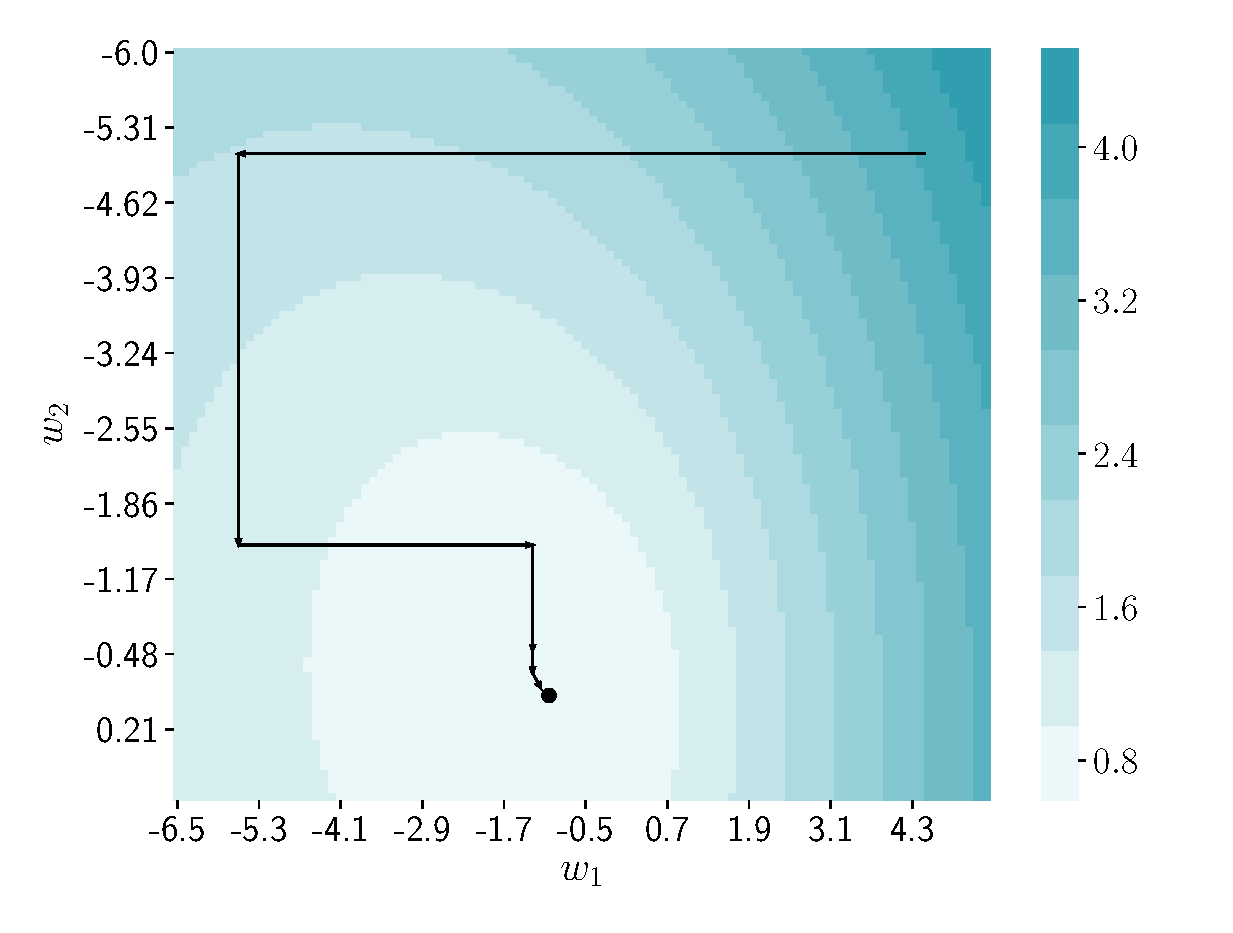
\includegraphics[width=0.6\linewidth]{figs/irls_qpfs_2d.eps}	 
  		\caption{Optimization process for logistic regression with QPFS+Newton algorithm}
  		\label{fig:irls_qpfs_2d}
  	\end{figure}
  	
  	\hrulefill
  
  We fitted the linear model for this data.
  The error landscape is shown in the figure~\ref{fig:linear_error} for two randomly selected weights. 
  We add the random noise to the optimum weights $\bw^*$ to get the point $\bw^0$. The behaviour of the Rel term vector $\bb$ on the line segment between $\bw^0$ and $\bw^*$ is illustrated in the figure~\ref{fig:linear_b_wrt_beta}.

	\begin{figure}[!h]	
		\centering
		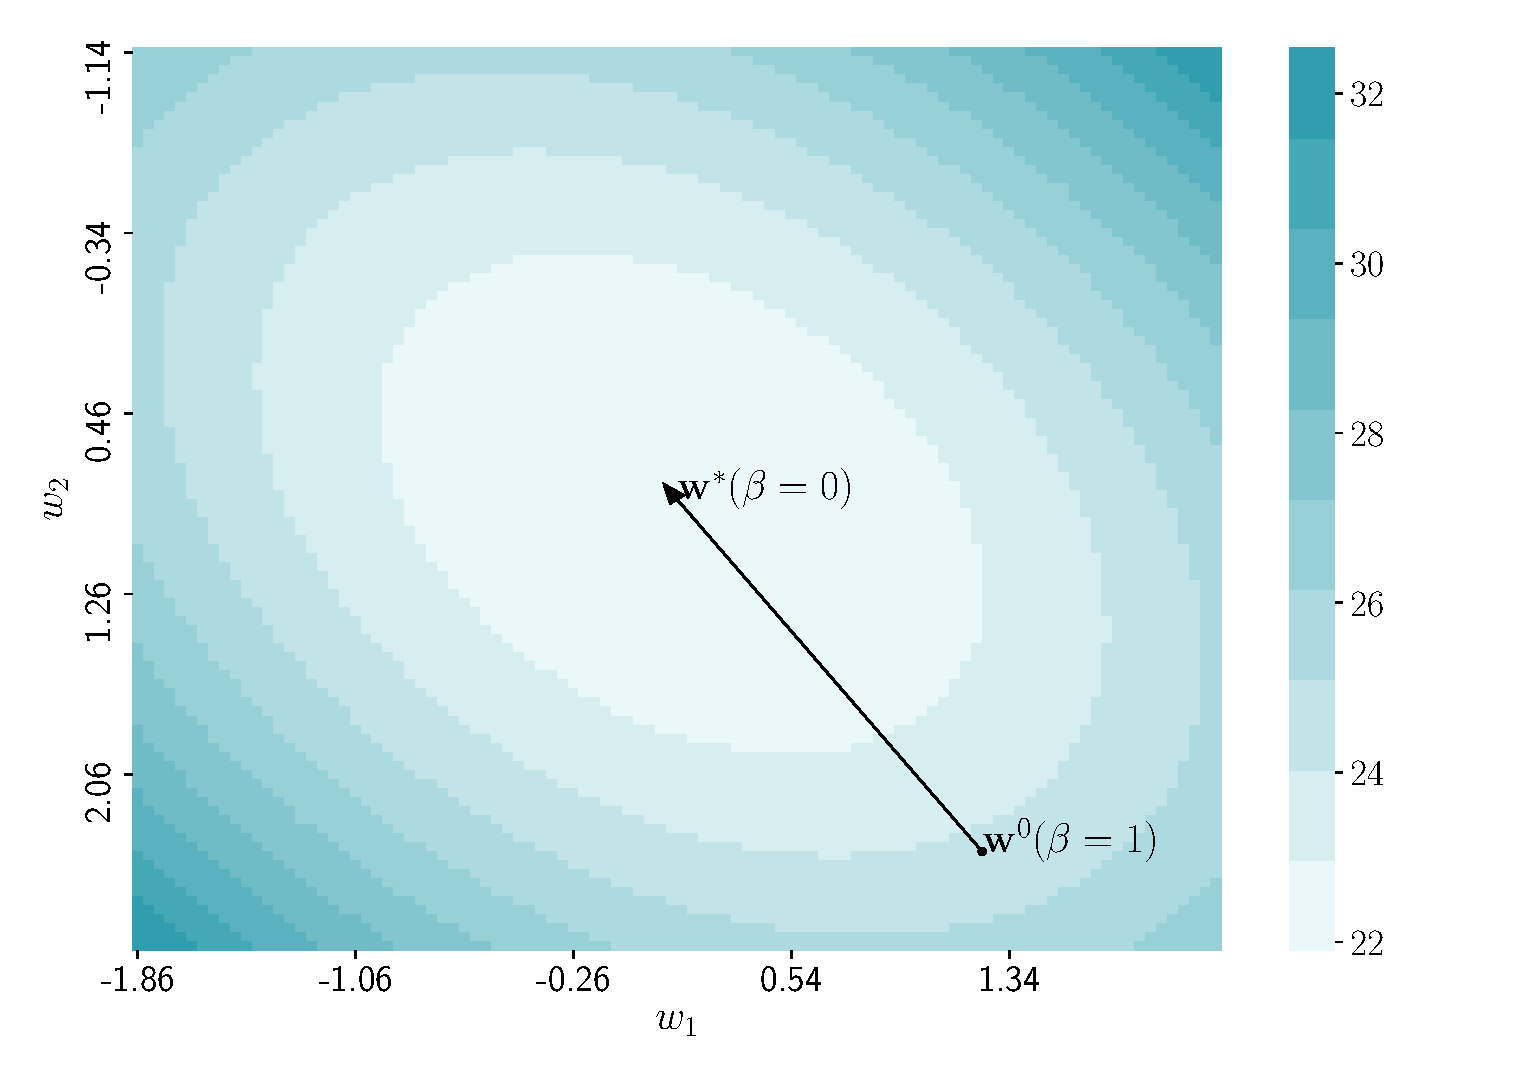
\includegraphics[width=0.8\linewidth]{figs/linear_error.eps}	 
		\caption{Error function landscape near optimal weight point for linear model.}
		\label{fig:linear_error}
	\end{figure}

	\begin{figure}[!h]	
		\centering
		\includegraphics[width=\linewidth]{figs/linear_b_wrt_beta.eps}	 
		\caption{Relevance scores for linear model with respect to $\beta$ coefficient.}
		\label{fig:linear_b_wrt_beta}
	\end{figure}

	The landscape for the neural network model is more complex. We use only 2 hidden units to get not excessively complex model.
	The optimal weight vector $\bw^*$ is obtained by backpropagation optimization procedure. 
	Figure~\ref{fig:neural_error} shows the error function on the grid of two neural network weights from~$\bW_1$. 
	We use the same strategy to investigate how the linear term vector $\bb$ is changing moving from $\bw^0$ to $\bw^*$. 
	The result are shown in the figure~\ref{fig:neural_b_wrt_beta}.
	

	\begin{figure}[!h]	
		\centering
		\includegraphics[width=0.8\linewidth]{figs/neural_error.eps}	 
		\caption{Error function landscape near optimal weight point for neural network.}
		\label{fig:neural_error}
	\end{figure}
	
	\begin{figure}[!h]	
		\centering
		\includegraphics[width=\linewidth]{figs/neural_b_wrt_beta.eps}	 
		\caption{Relevance scores for neural network with respect to $\beta$ coefficient.}
		\label{fig:neural_b_wrt_beta}
	\end{figure}
				
   \newpage
   \hrulefill
  
	\end{document}